% Rekonstruierte main.tex aus dem PDF "AP1 V36-1.pdf"
% Universität Freiburg – Physiklabor für Anfänger*innen 1
\documentclass[12pt,a4paper]{article}

\usepackage[T1]{fontenc}
\usepackage[utf8]{inputenc}
\usepackage[ngerman]{babel}
\usepackage{lmodern}
\usepackage{amsmath,amssymb,amsthm}
\usepackage{graphicx}
\usepackage{float}
\usepackage[a4paper,margin=3cm]{geometry}
\usepackage{setspace}
\usepackage{siunitx}
\usepackage{booktabs}
\usepackage{tabularx}
\usepackage{hyperref}
\usepackage{cleveref}
\usepackage{csquotes}

\onehalfspacing
\setlength{\parindent}{0pt}
\setlength{\parskip}{0.4em}

\sisetup{
  locale = DE,
  separate-uncertainty = true,
  per-mode = symbol
}

\hypersetup{
  hidelinks
}

\begin{document}

\begin{titlepage}
    \centering
    \vspace*{2cm}

    {\Large Universität Freiburg\par}
    \vspace{0.5cm}
    {\large Physiklabor für Anfänger*innen 1\par}
    \vspace{1cm}
    {\large Ferienpraktikum im Sommersemester 2026\par}

    \vspace{2cm}

    {\huge\bfseries Versuch 36\par}
    \vspace{0.5cm}
    {\LARGE Adiabatenexponent\par}

    \vfill

    {\large
    Lorenz Klug, Matti Jacob, Oskar Gentner\\
    (Gruppe 143)
    \par}

    \vspace{1cm}

    {\large
    24.09.2026\\
    Datum der Durchführung: 23.09.2026\\
    Assistent*in: Alex
    \par}
\end{titlepage}

\tableofcontents
\newpage

\section{Ziel des Versuchs}

Wir bestimmen die Adiabatenexponenten von Luft und Helium und deren Freiheitsgrade mithilfe eines Aufbaus nach Rüchardt/Flammersfeld.

\section{Versuchsdurchführung}

Für den Aufbau nutzen wir einen Glaskolben mit Präzisionsrohr, in welchem sich ein Schwingkörper befindet. Das Rohr hat ein seitliches kleines Loch (1 in \cref{fig:versuchsaufbau}), durch welches Gas entweichen kann. Durch ein Nadelventil wird das jeweilige Gas oder Gasgemisch in den Kolben gepumpt, wodurch der Schwingkörper nach oben gedrückt wird. Sobald er sich über der Öffnung 1 befindet, kann das Gas dadurch entweichen und der Körper fällt wieder nach unten und schließt das Loch. Hierdurch entsteht eine näherungsweise harmonische Schwingung. Die Schwingdauern $T_n$ werden anhand des induzierten Stroms in einer an dem Präzisionsrohr angebrachten Spule gemessen.

Im ersten Versuchsdurchgang wird der Adiabatenexponent $\gamma_L$ von Luft und dessen Freiheitsgrade $f_L$ durch $T_n$-Messungen über $n$ Perioden berechnet. Anschließend wird der Versuch mit Helium durchgeführt und es werden auf gleiche Weise $\gamma_{\mathrm{He}}$ sowie die Freiheitsgrade $f_{\mathrm{He}}$ bestimmt.

\begin{figure}[H]
    \centering
    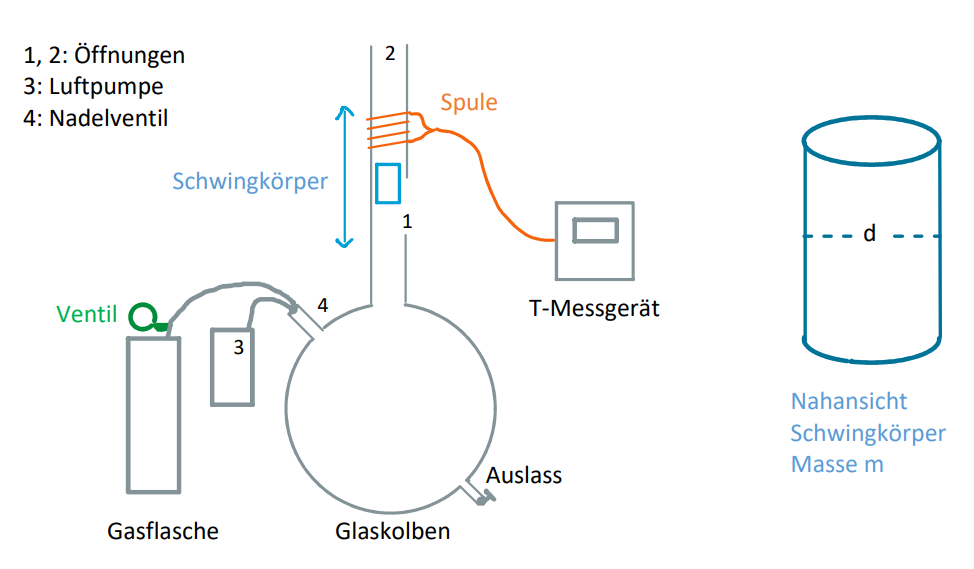
\includegraphics[width=0.85\textwidth]{abb01_versuchsaufbau.png}
    \caption{Versuchsaufbau}
    \label{fig:versuchsaufbau}
\end{figure}

\section{Auswertung und Fehleranalyse}

\subsection{Umgebungsbedingungen}

Der verwendete Glaskolben besitzt das Volumen
$$
V=(2220\pm10)\cdot10^{-6}\,\si{\meter\cubed}.
$
Die lokale Erdbeschleunigung ist gegeben als
$$
g=(9{,}808\pm0{,}001)\,\si{\meter\per\second\squared}.
$$
Der umgebende Luftdruck beträgt
$$
p_L=(99050\pm20)\,\si{\pascal}
$$
(Quecksilber-Barometer, Dreiecksverteilung mit $2a=\SI{100}{Pa}$).

Der Durchmesser des Schwingkörpers beträgt
$$
d=(13{,}8\pm0{,}02)\,\si{\milli\meter}
$$
(Messschieber, Dreiecksverteilung mit $2a=\SI{0.05}{mm}$) und seine Masse
$$
m=(5{,}67\pm0{,}006)\,\si{\gram}
$$
(Digitalwaage, Dreiecksverteilung mit $2a=\SI{0.01}{g}$).

Die intrinsische Ungenauigkeit der Zeitstoppuhr beträgt
$$
\Delta T=\SI{0.002}{s}
$$
(Rechtecksverteilung mit $2a=\SI{0.01}{s}$). Die menschliche Unsicherheit durch das händische Stoppen $\Delta T_i$ entspricht einer Schwingungsperiode
$$
\Delta T_i=\frac{T_i}{n_i}.
$$

\subsection{Versuch mit Luft}

Die Luftpumpe wird an das Nadelventil angeschlossen und füllt den Glaskolben.

\subsubsection{Bestimmung der Schwingungsdauer von zehn Perioden $\bar{T}_{10}$}

Um den Mittelwert der Schwingungen $\bar{T}_{10}$ zu bestimmen, messen wir fünfzig mal jeweils zehn Perioden $T_{10}$. Die Messdaten sind im folgendem Histogramm eingetragen.

\begin{figure}[H]
    \centering
    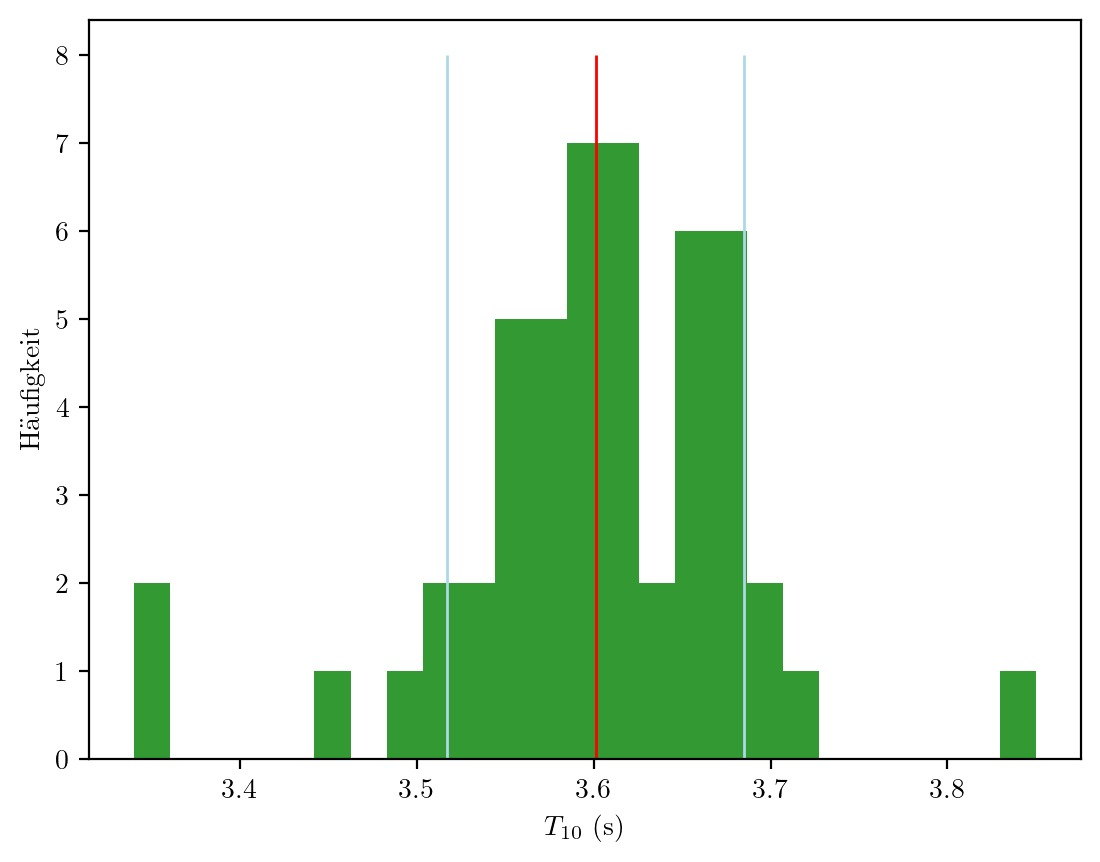
\includegraphics[width=0.85\textwidth]{abb02_histogramm_T10_luft.jpg}
    \caption{Histogramm der Messung von $T_{10}$ mit Mittelwert (rot) und Standardabweichung (hellblau)}
    \label{fig:histogramm}
\end{figure}

Aufgrund der Form lässt sich eine Normalverteilung annehmen. Es werden rechnerisch der Mittelwert
\[
\bar{T}_{10}=\SI{3.60}{s}
\]
sowie die Standardabweichung
\[
s_{T10}=\SI{0.084}{s}
\]
bestimmt.

\subsubsection{Bestimmung der Periodendauer einer Schwingung $\bar{T}_L$}

Um den Mittelwert einer Periodendauer $\bar{T}_L$ zu bestimmen, messen wir die Schwingungsdauer für mehrere verschiedene Periodenzahlen $n$ je einmal. Aus diesen Daten erhalten wir die Werte in Tabelle 1 und folgendem Diagramm.

\begin{figure}[H]
    \centering
    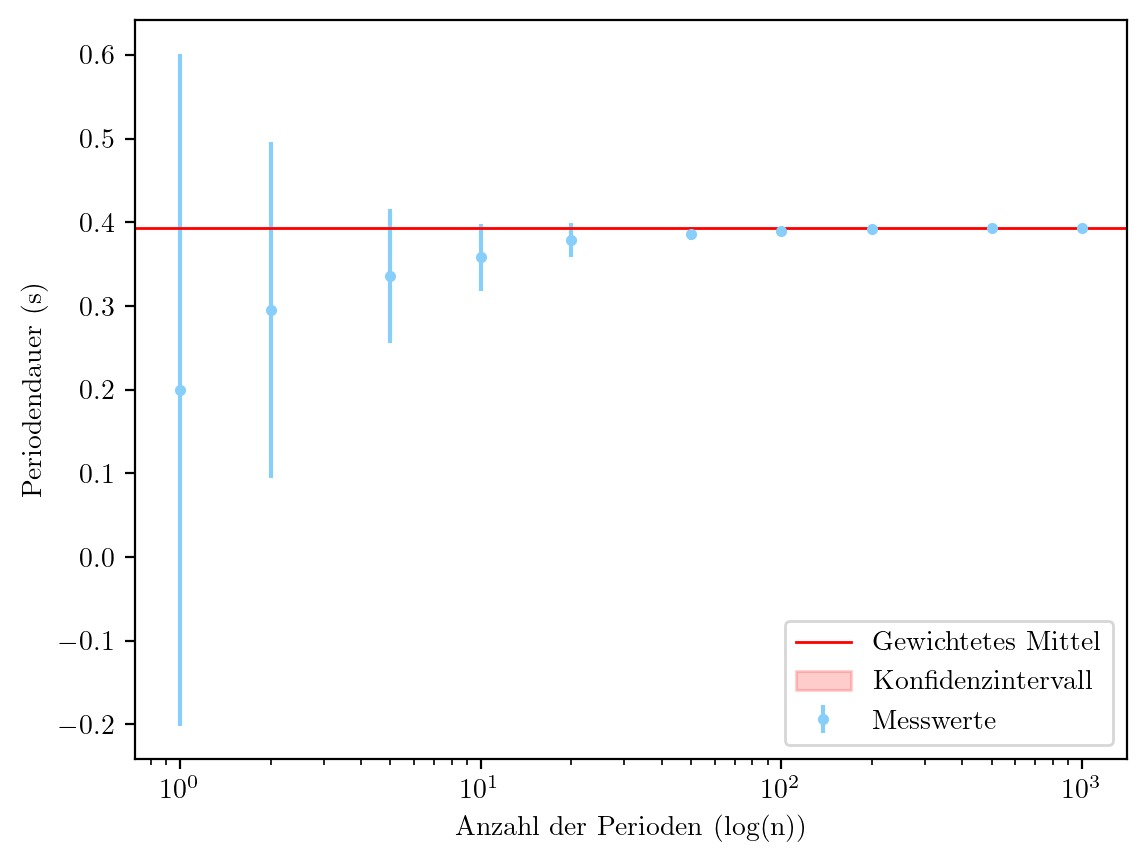
\includegraphics[width=0.85\textwidth]{abb03_periodendauer_luft.jpg}
    \caption{Diagramm einer einzelnen Periodendauer für Luft gegen die Anzahl der gemessenen Perioden mit logarithmischer $x$-Achse, gewichtetem Mittelwert (rot) und Unsicherheiten (vertikale Balken)}
    \label{fig:luft-periodendauer}
\end{figure}

Der gewichtete Mittelwert $\bar{T}_L$ lässt sich durch\footnote{Datenanalyse A, Formel A.33, A.34}
\[
\bar{T}_L=
\frac{\displaystyle\sum_{i=1}^{10}\omega_i T_i}
{\displaystyle\sum_{i=1}^{10}\omega_i}
\quad\text{mit}\quad
\omega_i=\frac{1}{\Delta x_i}
\tag{1}
\]
berechnen, was dem Wert
\[
\bar{T}_L=\SI{0.39}{s}
\]
entspricht.

Die Fehler der einzelnen Messungen berechnen sich durch
\begin{equation}
\Delta T_n=
\sqrt{
\left(\frac{s_{T10}}{n}\right)^2+
\left(\frac{\bar{T}_L}{n}\right)^2
}.
\tag{2}
\end{equation}

Deutlich zu erkennen ist, dass die Messungen über viele Perioden eine geringere Unsicherheit pro Periode haben und den gewichteten Mittelwert $\bar{T}_L$ dominant beeinflussen.

\subsubsection{Bestimmung des Adiabatenexponenten von Luft $\gamma_L$}

Um den Adiabatenexponenten bestimmen zu können, nutzen wir die Formel\footnote{Schenk, Physikalisches Praktikum, Formel (43)}
\begin{equation}
\gamma=
\frac{64mV}{\bar{T}^{\,2}d^4p}.
\tag{3}
\end{equation}
mit\footnote{Schenk, Physikalisches Praktikum, Seite 136}
\begin{equation}
p=p_L+\frac{4mg}{\pi d^2}.
\tag{4}
\end{equation}

Durch diese Formel erhalten wir den Wert
\[
\gamma_L=1{,}45\pm0{,}01,
\]
wobei der Fehler in Abschnitt 3.6 berechnet wird.

\subsection{Bestimmung der Freiheitsgrade $f_L$}

Um die Freiheitsgrade $f_L$ zu bestimmen, gehen wir statistisch vor. Der theoretische Wert des Adiabatenexponenten lässt sich errechnen durch
\begin{equation}
\gamma=\frac{f+2}{f}.
\tag{5}
\end{equation}

Zur Visualisierung hilft folgender Graph. [einheitliche Farben verwenden]

\begin{figure}[H]
    \centering
    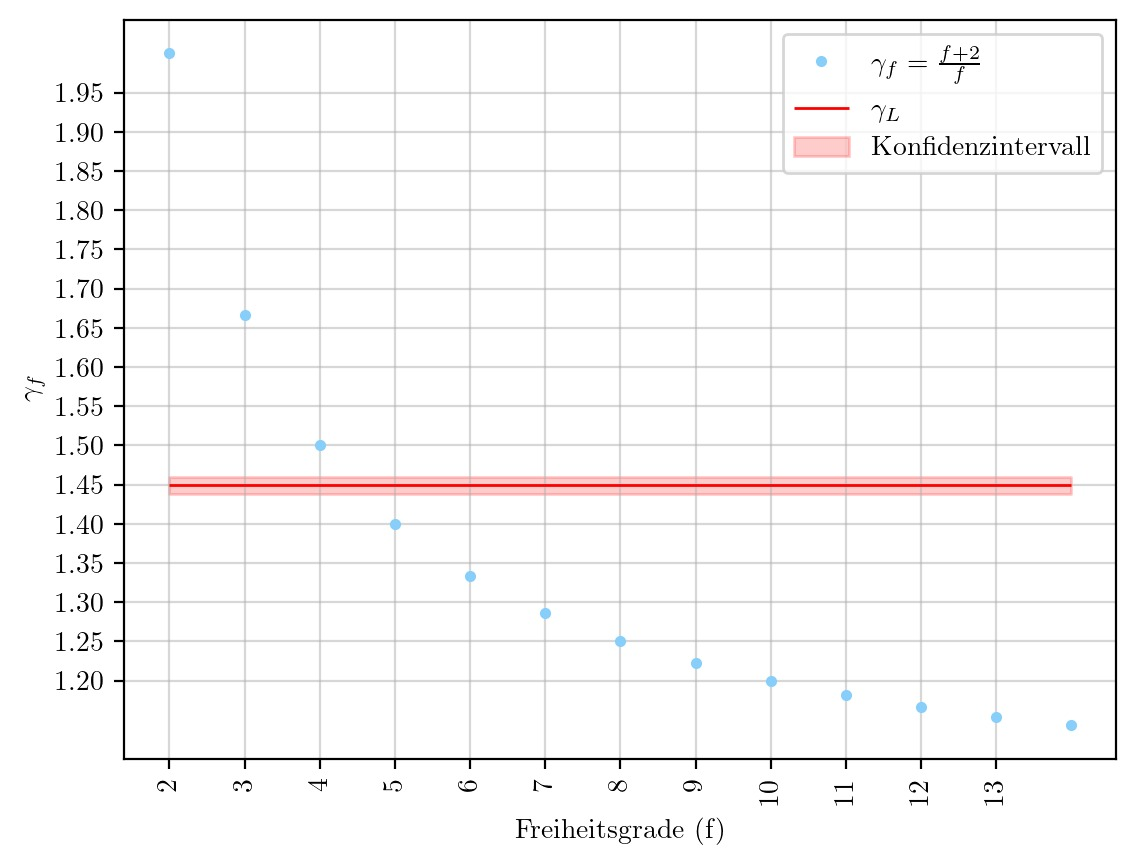
\includegraphics[width=0.85\textwidth]{abb04_gamma_freiheitsgrade_luft.jpg}
    \caption{Der Adiabatenexponent für verschiedene Freiheitsgrade $\gamma_f$ (blau) und unser errechneter Adiabatenexponent $\gamma_L$ (rot)}
    \label{fig:gamma-f-luft}
\end{figure}

Wir erkennen hier, dass keiner der Freiheitsgrade auf unserem berechneten $\gamma_L$ liegt.

Mithilfe des $z$-Tests lässt sich veranschaulichen, welche Freiheitsgrade mit unserem Adiabatenexponenten verträglich sind. Wir berechnen die $z$-Werte mit
\begin{equation}
|z|=\frac{|\bar{\gamma}-\gamma_f|}{\Delta\gamma}.
\tag{6}
\end{equation}

\begin{figure}[H]
    \centering
    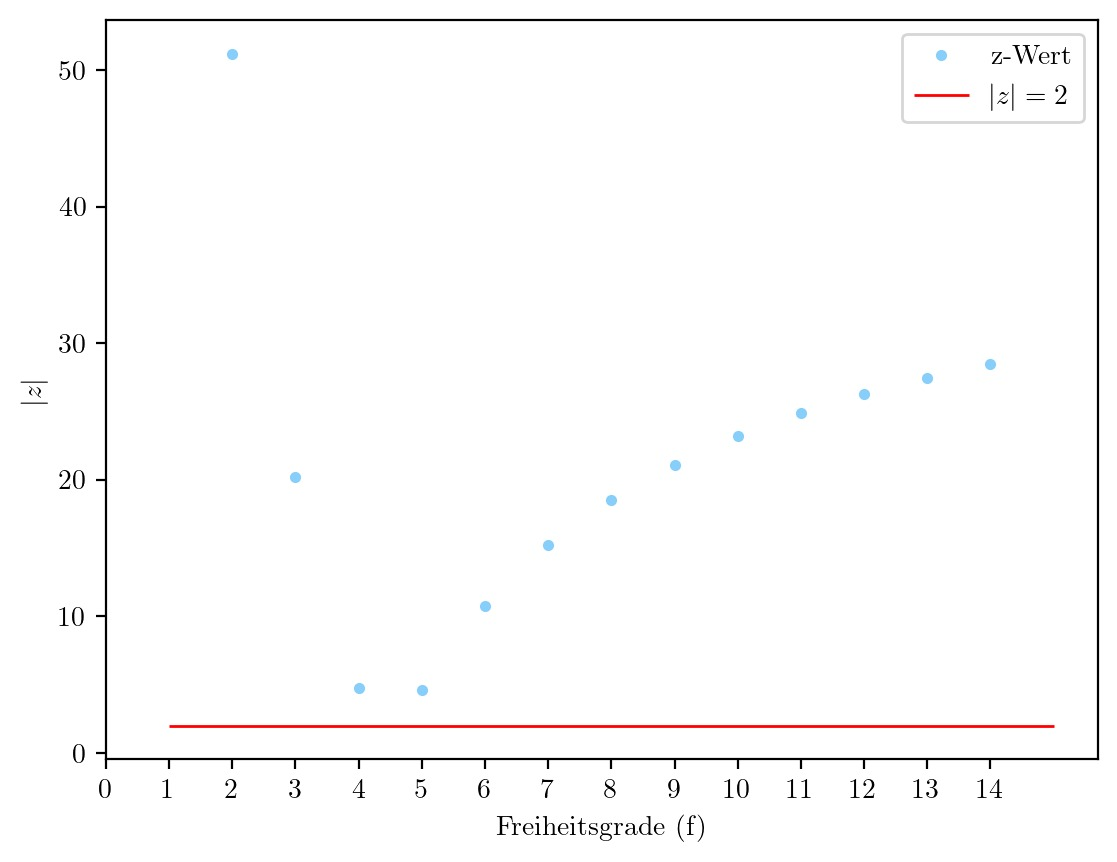
\includegraphics[width=0.85\textwidth]{abb05_zwerte_luft.jpg}
    \caption{$z$-Werte für die jeweiligen $\gamma_f$ (grün), Signifikanzniveau $|z|=2$ (rot)}
    \label{fig:z-luft}
\end{figure}

Keiner der $z$-Werte liegt unterhalb des Signifikanzniveaus, es ist also kein Freiheitsgrad mit unserem Adiabatenexponenten für Luft vereinbar.

\subsection{Versuch mit Helium}

Nun wird der Glaskolben von der Luftpumpe getrennt und an die Heliumflasche angeschlossen. Allerdings messen wir jetzt direkt verschiedene Periodenzahlen, welche in Tabelle 2 einzusehen sind.

\subsubsection{Bestimmung der Periodendauer einer Schwingung $\bar{T}_{\mathrm{He}}$}

Wie in Abschnitt 3.2.2 führen wir Messungen der Schwingungsdauer für $n$ viele Perioden durch. Diese sind analog zu oben im folgenden Diagramm aufgetragen.

\begin{figure}[H]
    \centering
    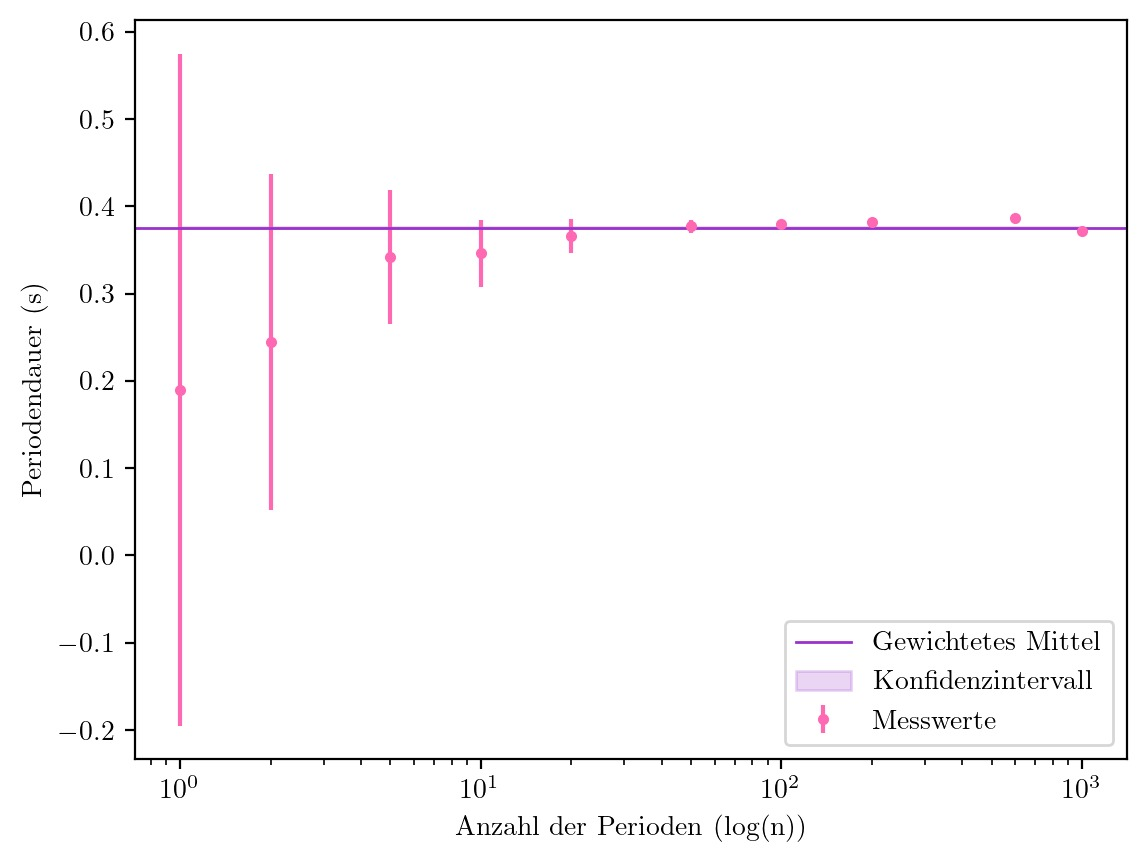
\includegraphics[width=0.85\textwidth]{abb06_periodendauer_helium.jpg}
    \caption{Diagramm einer einzelnen Periodendauer für Helium gegen die Anzahl der Perioden mit logarithmischer $x$-Achse, gewichtetem Mittelwert (Farbe) und Unsicherheiten (vertikale Balken)}
    \label{fig:helium-periodendauer}
\end{figure}

Wie zu erwarten hat der Graph Ähnlichkeiten zu Abb. 3, wobei auffällt, dass $T_{600}$ unerwartet weit entfernt vom gewichteten Mittelwert $\bar{T}_{\mathrm{He}}=\SI{0.376}{s}$ liegt. Die Standardabweichung $s_{\bar{T}_{\mathrm{He}}}$ ist von der Größenordnung $10^{-5}$ und wird vernachlässigt.

\subsubsection{Bestimmung des Adiabatenexponenten von Helium $\gamma_{\mathrm{He}}$}

Der Adiabatenexponent wird wie in Abschnitt 3.2.3 berechnet. Dadurch erhalten wir den Wert
\[
\gamma_{\mathrm{He}}=1{,}58\pm0{,}01.
\]
Der Fehler ist in Abschnitt 3.6.2 berechnet.

\subsection{Bestimmung der Freiheitsgrade $f_{\mathrm{He}}$}

Auch hier arbeiten wir mit Gleichung (5), um die Freiheitsgrade $f_{\mathrm{He}}$ von Helium zu bestimmen. Wir bilden die Ergebnisse in folgendem Diagramm ab.

\begin{figure}[H]
    \centering
    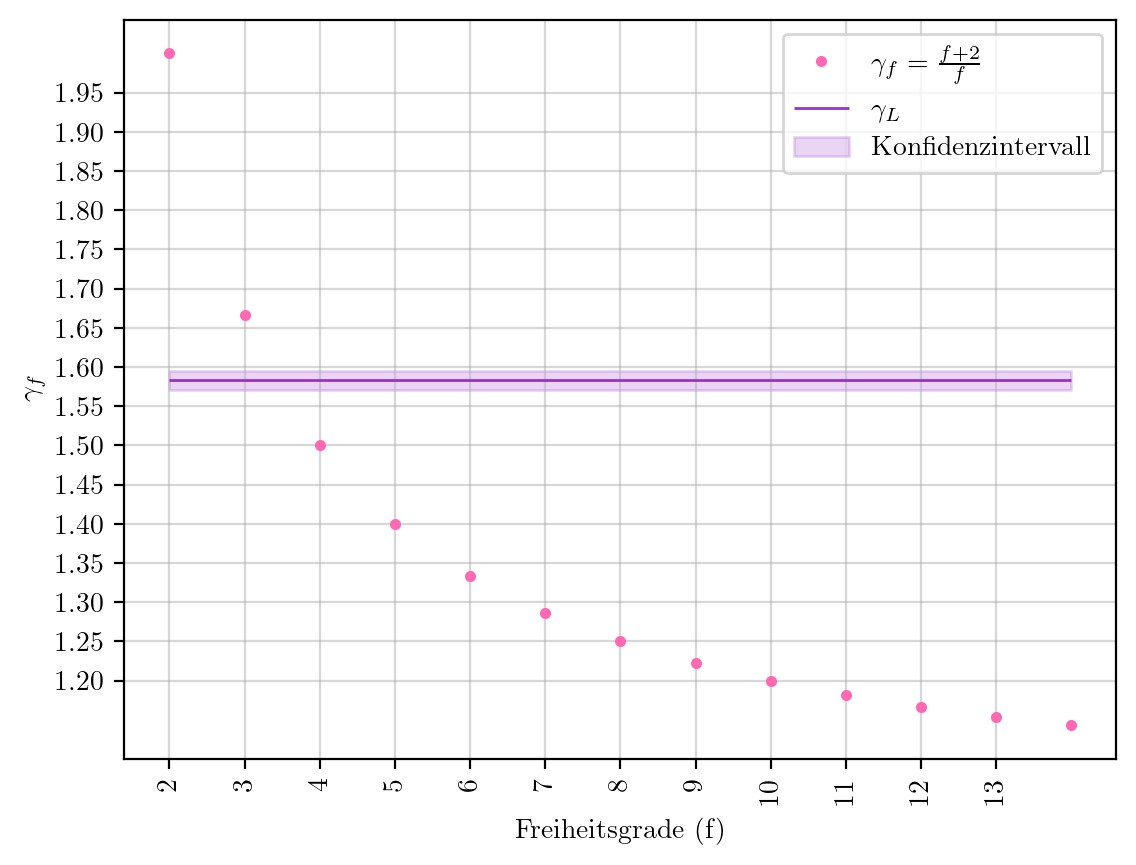
\includegraphics[width=0.85\textwidth]{abb07_gamma_freiheitsgrade_helium.jpg}
    \caption{Adiabatenexponent gegen die Anzahl der Freiheitsgrade mit theoretischem Wert nach gegebener Formel (blau) und dem durch unsere Messungen berechneten (rot)}
    \label{fig:gamma-f-helium}
\end{figure}

Es befindet sich kein ganzzahliger Wert $\gamma_f$ auf unserer Geraden für $\gamma_{\mathrm{He}}$. Das widerspricht unserer Erwartung für ein reines Gas. Wir führen auch hier den $z$-Test durch und prüfen die Verträglichkeit unserer Ergebnisse in folgendem Diagramm.

\begin{figure}[H]
    \centering
    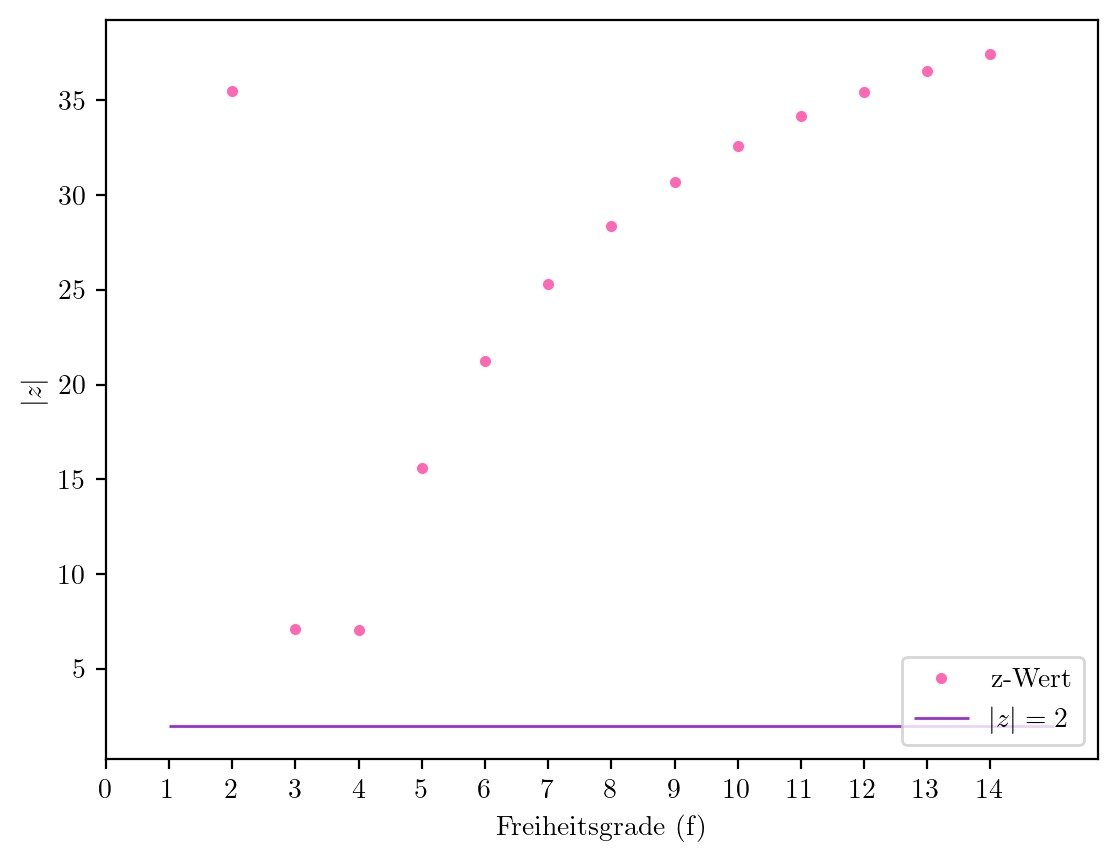
\includegraphics[width=0.85\textwidth]{abb08_zwerte_helium.jpg}
    \caption{$z$-Werte für die jeweiligen $\gamma_f$ (grün) mit Signifikanzniveau $|z|=2$ (rot)}
    \label{fig:z-helium}
\end{figure}

Es fällt auf, dass ebenfalls keiner der $\gamma_f$-Werte unterhalb des Signifikanzniveaus liegt, also kein Wert mit unserem Ergebnis für $\gamma_{\mathrm{He}}$ verträglich ist.

Die Freiheitsgrade $f=3,4$ liegen hierbei am nächsten zu $|z|=2$. Da in beiden Messungen keiner der Adiabatenexponenten mit einem Freiheitsgrad übereinstimmt, ist naheliegend, dass ein unbeachteter systematischer Fehler unsere Ergebnisse verfälscht.

\subsection{Fehlerfortpflanzung}

\subsubsection{Fehlerfortpflanzung von $\gamma_L$}

Wir verwenden die Gauß'sche Fehlerfortpflanzung (Gleichung (7)) mit $T=\bar{T}_L$, um den Fehler von $\gamma_L$ zu bestimmen. Wir haben Unsicherheiten auf allen Parametern und benötigen fünf Fehlerterme unter der Wurzel (Gleichung (8) und folgende).

Wir erhalten:
\[
\Delta\gamma_L=0{,}01.
\]

Dabei dominieren der $V$-Term $=4\cdot10^{-5}$ und der $d$-Term $=7\cdot10^{-5}$.

\subsubsection{Fehlerfortpflanzung von $\gamma_{\mathrm{He}}$}

$\Delta\gamma_{\mathrm{He}}$ wird wie $\Delta\gamma_L$ aus Gleichung (7) berechnet, allerdings mit $T=\bar{T}_{\mathrm{He}}$.

Wir erhalten auch für Helium:
\[
\Delta\gamma_{\mathrm{He}}=0{,}01.
\]

Es dominieren wieder der $V$-Term $=5\cdot10^{-5}$ und der $d$-Term $=8\cdot10^{-5}$.

Es ist zu beobachten, dass, obwohl die gleichen Terme den Fehler dominieren, deren Beträge für Helium um eine relevante Ziffer höher sind als für Luft.

\section{Diskussion}

\subsection{Ergebnisse und Vergleich mit dem Literaturwert}

Die von uns berechneten Adiabatenexponenten betragen für Luft
$$
\gamma_L=1{,}45\pm0{,}01
$$
und für Helium
$$
\gamma_{\mathrm{He}}=1{,}58\pm0{,}01.
$$

Literaturwerte\footnote{\url{https://de.wikipedia.org/wiki/Isentropenexponent}}
sind
$$
\gamma_L=1{,}40
$$
und
$$
\gamma_{\mathrm{He}}=1{,}67.
$$

Da es sich bei Luft um hauptsächlich mehratomige Gase handelt (Stickstoff, Sauerstoff), sollte es ungefähr $f=5$ Freiheitsgrade geben. Bei Helium handelt es sich um ein einatomiges Edelgas mit den Freiheitsgraden $f=3$.\footnote{\url{https://www.tec-science.com/de/thermodynamik-waermelehre/kinetische-gastheorie/innere-energie-molare-warmekapazitat/}, zuletzt aufgerufen: 24.09.2026, 11:30 Uhr}

Unsere Werte weichen signifikant von den Literaturwerten ab
$$
|z|_L=5>2,\qquad |z|_{\mathrm{He}}=9>2.
$$
Obwohl keiner unserer errechneten Adiabatenexponenten zu einem Freiheitsgrad passt, lässt sich im Graphen ablesen, dass die literarischen Freiheitsgrade am ehesten zu unseren Werten passen.

Das signifikante Abweichen könnte an mehreren Faktoren liegen. Zum einen haben wir nicht nach dem ersten Messen den Glaskolben durchgespült, wodurch vor allem der ausfallende Wert aus Abb. 9 erklärt wäre. Dieser ist nämlich vor der Durchspülung aufgezeichnet worden. Zudem könnte ein Fehler bei der Druckmessung passiert sein. Der Luftdruck zum Zeitpunkt der Messung war laut dem Meteorologischen Institut Freiburg\footnote{\url{https://weather.uni-freiburg.de/}} bei ca. $\SI{102400}{Pa}$, etwas höher als der von uns gemessene
$$
p_L=(99050\pm20)\,\si{\pascal}.
$$
Rechnet man mit dem Luftdruck des Meteorologischen Instituts, liegt unser Ergebnis für $\gamma_L$ innerhalb des Signifikanzniveaus.

\subsection{Störeinflüsse}

\begin{itemize}
    \item Wir können nicht sicherstellen, dass vor dem Befüllen des Kolbens mit Helium die Luft vollständig ausgespült wurde. Das hätte zur Folge, dass wir nicht mit reinem Helium, sondern einem Helium-Luft-Gemisch gearbeitet haben.
    \item Es ist möglich, dass Reibung des Schwingkörpers an der Innenwand des Präzisionsrohrs die Periodendauer beeinflusst.
    \item Der Luftdruck oder die Temperatur werden im Versuchsaufbau als konstant angenommen. Allerdings könnten durch offene Fenster die Temperatur und der Luftdruck schwanken, wodurch das Ergebnis verfälscht wird.
\end{itemize}

\subsection{Verbesserungsvorschläge}

Wir haben einige Verbesserungsvorschläge gesammelt, um eine präzisere Messung zu ermöglichen.

\begin{itemize}
    \item Eine große Ungenauigkeit entsteht durch die $T$-Messung. Zur Verbesserung würden ein Messgerät mit höherer Auflösung sowie ein automatisches Stoppen der Uhr, z.\,B. durch eine Lichtschranke, beitragen. Durch die Lichtschranke wäre auch das Stoppen der Uhr zur immer gleichen Phase der Schwingung gewährleistet.
    \item Es könnte außerdem ein Schwingkörper mit geringerer Seitenfläche verwendet werden, um die Reibung an den Wänden zu reduzieren.
    \item Da Temperatur und Luftdruck eine Rolle in diesem Experiment spielen, könnte man mit einem gut isolierten Raum diese Störfaktoren minimieren.
\end{itemize}

\section{Autorenschaft}

Alle Autoren haben zu allen Inhalten des Protokolls zu gleichen Teilen beigetragen.

\section{Anhang}

\subsection{Gauß'scher Fehler für $\gamma_L$}

Die allgemeine Formel lautet
\begin{align}
\Delta\gamma_L
={}&
\sqrt{
\left(
\frac{64V}{T^2d^4p}\Delta m
\right)^2
+
\left(
\frac{64m}{T^2d^4p}\Delta V
\right)^2
+
\left(
-\frac{128Vm}{T^3d^4p}\Delta T
\right)^2
\nonumber\\
&+
\left[
\left(
-\frac{256Vm}{T^2d^5p}
\right)
+
\left(
\frac{512Vm^2g}{\pi T^2d^7p^2}
\right)
\right]^2
(\Delta d)^2
+
\left(
-\frac{64Vm}{T^2d^4p^2}\Delta p
\right)^2
}.
\end{align}

Mit
\[
p=p_L+\frac{4mg}{\pi d^2}
\]
ergibt sich nach Einsetzen der Größen
\begin{align}
\Delta\gamma_L
={}&
\Bigg[
\left(
\frac{64V}{T^2d^4\left(p_L+\frac{1.27gm}{d^2}\right)}
-\frac{81.49Vgm}{T^2d^6\left(p_L+\frac{1.27gm}{d^2}\right)^2}
\right)\Delta m
\Bigg]^2
\nonumber\\
&+
\left(
-\frac{81.49Vm^2}{T^2d^6\left(p_L+\frac{1.27gm}{d^2}\right)^2}
\Delta g
\right)^2
\nonumber\\
&+
\left(
\frac{64m}{T^2d^4\left(p_L+\frac{1.27gm}{d^2}\right)}
\Delta V
\right)^2
\nonumber\\
&+
\Bigg[
\left(
-\frac{256Vm}{T^2d^5\left(p_L+\frac{1.27gm}{d^2}\right)}
+
\frac{162.97Vgm^2}{T^2d^7\left(p_L+\frac{1.27gm}{d^2}\right)^2}
\right)
\Delta d
\Bigg]^2
\nonumber\\
&+
\left(
-\frac{64Vm}{T^2d^4\left(p_L+\frac{1.27gm}{d^2}\right)^2}
\Delta p_L
\right)^2
\nonumber\\
&+
\left(
-\frac{128Vm}{T^3d^4\left(p_L+\frac{1.27gm}{d^2}\right)}
\Delta T
\right)^2
\Bigg]^{1/2}
=0{,}01.
\tag{7}
\end{align}

Einzelne Fehlerterme für Dominanzverhalten:
\begin{align}
m\text{-Term} &=
\left(
\frac{64V}{T^2d^4\left(p_L+\frac{1.27gm}{d^2}\right)}
-\frac{81.49Vgm}{T^2d^6\left(p_L+\frac{1.27gm}{d^2}\right)^2}
\right)^2
(\Delta m)^2
=2\cdot10^{-6},
\tag{8}\\
V\text{-Term} &=
\left(
\frac{64m}{T^2d^4\left(p_L+\frac{1.27gm}{d^2}\right)}
\Delta V
\right)^2
=4\cdot10^{-5},
\\
T\text{-Term} &=
\left(
-\frac{128Vm}{T^3d^4\left(p_L+\frac{1.27gm}{d^2}\right)}
\Delta T
\right)^2
=3\cdot10^{-7},
\\
d\text{-Term} &=
\Bigg[
\left(
-\frac{256Vm}{T^2d^5\left(p_L+\frac{1.27gm}{d^2}\right)}
+\frac{162.97Vgm^2}{T^2d^7\left(p_L+\frac{1.27gm}{d^2}\right)^2}
\right)
\Delta d
\Bigg]^2
=7\cdot10^{-5},
\\
p\text{-Term} &=
\left(
-\frac{64Vm}{T^2d^4\left(p_L+\frac{1.27gm}{d^2}\right)^2}
\Delta p_L
\right)^2
=8\cdot10^{-8},
\\
g\text{-Term} &=
\left(
-\frac{81.49Vm^2}{T^2d^6\left(p_L+\frac{1.27gm}{d^2}\right)^2}
\Delta g
\right)^2
=3\cdot10^{-13}.
\end{align}

\subsection{Gauß'scher Fehler für $\gamma_{\mathrm{He}}$}

Einzelne Fehlerterme für Dominanzverhalten (gleiche Formeln wie Gleichung (8) und folgende):
\begin{align*}
m\text{-Term} &=2\cdot10^{-6},&
V\text{-Term} &=5\cdot10^{-5},&
T\text{-Term} &=3\cdot10^{-7},\\
d\text{-Term} &=8\cdot10^{-5},&
p\text{-Term} &=1\cdot10^{-7},&
g\text{-Term} &=4\cdot10^{-13}.
\end{align*}

\subsection{Messdaten}

\begin{table}[H]
\centering
\caption{Periodendauern Luft für unterschiedliche $n$}
\begin{tabular}{rrr}
\toprule
Perioden $n$ & Dauer (s) & Periodendauer (s)\\
\midrule
1 & 0,20 & 0,20\\
2 & 0,59 & 0,295\\
5 & 1,68 & 0,336\\
10 & 3,58 & 0,358\\
20 & 7,58 & 0,379\\
50 & 19,32 & 0,3864\\
100 & 38,95 & 0,3895\\
200 & 78,33 & 0,39165\\
500 & 196,37 & 0,39274\\
1000 & 392,70 & 0,3927\\
\bottomrule
\end{tabular}
\end{table}

\begin{table}[H]
\centering
\caption{Periodendauern He für unterschiedliche $n$}
\begin{tabular}{rrr}
\toprule
Perioden $n$ & Dauer (s) & Periodendauer (s)\\
\midrule
1 & 0,19 & 0,19\\
2 & 0,49 & 0,245\\
5 & 1,71 & 0,342\\
10 & 3,46 & 0,346\\
20 & 7,32 & 0,366\\
50 & 18,85 & 0,377\\
100 & 38 & 0,38\\
200 & 76,36 & 0,3818\\
600 & 231,92 & 0,38653333\\
1000 & 371,48 & 0,37148\\
\bottomrule
\end{tabular}
\end{table}

\begin{figure}[H]
    \centering
    \includegraphics[width=0.85\textwidth]{abb09_periodendauer_helium_anhang.jpg}
    \caption{Diagramm einer einzelnen Periodendauer für Helium gegen die Anzahl der Perioden mit logarithmischer $x$-Achse, gewichtetem Mittelwert (Farbe) und Unsicherheiten (vertikale Balken)}
    \label{fig:anhang-helium}
\end{figure}

\section{Labornotizen}

\end{document}
